% New manuscript. Existing reachability and mapping manuscripts are untouched.
% Offline evidence only; see README.md and evidence_audit.md before submission.
\documentclass[letterpaper,10pt,conference]{ieeeconf}
\IEEEoverridecommandlockouts
\overrideIEEEmargins
\usepackage{amsmath,amssymb,graphicx,booktabs,array,cite,url,xcolor}
\graphicspath{{figures/}}
\newcommand{\R}{\mathbb{R}}
\newcommand{\norm}[1]{\left\lVert #1\right\rVert}
\newcommand{\method}{cluster-centered dual-graph planning}
\newcommand{\draftnote}{\textit{Research draft: offline evidence; integrated task evaluation pending.}}
\title{\LARGE\bf From Semantic Clusters to Pre-Grasp Poses:\\
Coupling Environment Topology with Configuration Witnesses}
\author{Anonymous Authors}
\begin{document}
\maketitle
\thispagestyle{empty}\pagestyle{empty}

\begin{abstract}
A semantic object can overlap a robot's positional workspace while admitting no suitable gripper approach. We study this gap in a dual-graph manipulation prototype: a YOLOX-conditioned dynamic-density Growing Neural Gas graph represents observed objects and obstacles, while a separate roadmap retains archived numerical inverse-kinematic configurations and their end-effector poses. An object's observed cluster center supplies the target reference; pose-dependent stand-off, approach alignment, and sampled collision validation determine admissible robot goals. Our central distinction is between an object's geometric reference, the robot's attainable pre-grasp pose, and the collision geometry that must remain protected. An offline audit of 33,401 Cartesian grid queries finds 15,175 position witnesses but only 3,198 conditioning-qualified full-pose witnesses under the recorded scan policy. Independent forward kinematics verifies that every selected witness's end-effector local $+X$ lies within $0.44^\circ$ of world-down under the archived model, despite the gripper-frame orientation being specified as horizontal and radial. The bank therefore cannot justify horizontal local-$+X$ approach coverage. We derive this mismatch, specify a target-conditioned query contract, and document implementation limits. These results do not establish physical grasp success, improved planning performance, or continuous collision safety.
\end{abstract}

\section{Introduction}
An operator selects a bottle in an RGB-D scene and expects a manipulator to approach its body from the front. Three apparently reasonable decisions can defeat this intent. First, choosing the nearest labeled surface node can favor the bottle cap rather than its body. Second, a workspace point may have an inverse-kinematic witness whose orientation is unsuitable for approach. Third, a short end-effector path may carry the wrist, fingers, or camera through an obstacle. Semantic detection, position reachability, and whole-robot motion feasibility are different predicates.

We investigate their interaction using two representations. The environment graph $G_E$ summarizes observed geometry and semantic evidence. The robot graph $G_R$ stores joint configurations, forward-kinematic poses, and candidate transitions. Coupling these representations supports repeated target queries without treating environment edges as robot motions or discarding the configurations behind reachable positions. Our target is a \emph{pre-grasp pose}: a collision-checked configuration facing an object at a stand-off distance. Finger closure, contact, insertion, lift, and transport require additional task stages.

The motivating prototype previously used individual object nodes as target references. We replace that choice in the experiment launch with the midpoint of each same-class connected component's axis-aligned bounds. This point describes the observed cluster's spatial extent; it is neither an observed surface point nor a measured center of mass. Retaining a representative node identifier allows temporal association without forcing the physical reference to coincide with that node.

An implementation and data audit revealed a more fundamental issue than target-node selection. The archived workspace scan specifies orientations in a gripper frame and converts them to the end-effector control frame. A subsequent planner setting interpreted the control frame's local $+X$ as the gripper's forward axis. Those conventions differ. Changing a target to the cluster center, redrawing an arrow, or restarting a process cannot repair this geometric mismatch.

This paper makes three contributions at the prototype and offline-analysis level: (i) a cluster-centered target formulation that separates semantic identity, geometric reference, and protected collision geometry; (ii) an explicit coupling between that reference and a configuration-witness roadmap through pose-dependent goal predicates; and (iii) a reproducible workspace and frame-convention audit that identifies why positional overlap and local-axis alignment can still produce the wrong approach. The individual graph-learning, roadmap, and collision algorithms are established methods. The empirical contribution here is the analysis of the recorded witness bank, not a completed manipulation benchmark.

\section{Related Work}
Growing Neural Gas adapts a graph representation through competitive learning and node insertion~\cite{fritzke1995gng}. Dynamic-density GNG has been used with attention over topological representations for locomotion~\cite{saputra2023ddgng}. Our environment backend adapts its strength mechanisms using semantic evidence and bounded sampling; this is not a replication of the locomotion method. YOLOX supplies image-space class hypotheses~\cite{ge2021yolox}. Depth and visibility gates support their association to observed 3-D nodes, but image boxes alone do not provide instance masks or resolve all overlapping labels.

Capability maps expose position and orientation structure in robot workspaces~\cite{zacharias2007capability}. Probabilistic roadmaps retain configurations and reusable local transitions~\cite{kavraki1996prm}, while experience graphs reuse prior planning experience~\cite{phillips2012egraphs}. Our imported graph contains selected numerical IK witnesses from an archived scan. It does not store demonstrated physical trajectories, enumerate every IK branch, or preserve a learned environmental topology as motion connectivity.

Lazy PRM postpones expensive validation until candidate paths are queried~\cite{bohlin2000lazyprm}. We use a related reject-and-replan pattern with capsule checks and detailed robot geometry through MoveIt and FCL~\cite{coleman2014moveit,pan2012fcl}. OMPL provides established motion-planning infrastructure and suitable comparison baselines~\cite{sucan2012ompl}. Detailed geometry checks at discrete interpolated states must be distinguished from continuous collision detection.

Scene graphs can support task and motion planning over structured environments~\cite{ray2024scenegraph}. Here, semantic connectivity identifies an observed object component, whereas robot edges describe transitions in configuration space. The proposed interface concerns geometric pre-grasp queries, rather than symbolic task planning. We claim neither a new general scene-graph representation nor the first use of paired workspace and configuration-space representations.

\section{Problem Formulation}
Let $q\in\mathcal Q\subset\R^6$ satisfy the joint limits of a six-axis manipulator. The end-effector control frame $T$ has pose
\begin{equation}
 {}^WT_T(q)=\begin{bmatrix}R(q)&p(q)\\0&1\end{bmatrix},
 \quad R(q)\in SO(3),\quad p(q)\in\R^3.
\end{equation}
Frame $W$ is the world frame. A separate gripper convention $G$ may be related to $T$ by a fixed rotation. An approach axis must therefore be expressed in a specified frame, not just named ``$X$''.

\subsection{Observed Object Reference}
An environment node stores $u_j=(s_j,\ell_j,\gamma_j,\iota_j)$: observed world position, semantic class, confidence score, and identifier. Environment edges connect learned neighboring nodes. For a selected same-class connected component $C_k$, define the component-wise bounds and center
\begin{equation}
 b_{k,d}^{-}=\min_{j\in C_k}s_{j,d},\quad
 b_{k,d}^{+}=\max_{j\in C_k}s_{j,d},\quad
 c_{k,d}=\tfrac12(b_{k,d}^{-}+b_{k,d}^{+}).
 \label{eq:center}
\end{equation}
The identifier of the node nearest $c_k$ is retained only for association. Different disconnected components are not averaged together. Detector-instance tracking uses arithmetic centroids and temporal smoothing, while the coordinator also computes a confidence-weighted component centroid for association. These quantities remain distinct from the target in Eq.~\eqref{eq:center}.

This estimator avoids directly selecting a cap or side node merely because it is closest to the robot. It is still sensitive to outliers and incomplete views: a one-sided point cloud does not identify an object's hidden volume center. Same-class objects connected by erroneous graph edges may also merge. We therefore call $c_k$ the \emph{observed cluster center}, not the physical grasp center.

\subsection{Pose-Dependent Intersection}
Robot vertex $v_i$ retains $(q_i,p_i,R_i)$, with $(p_i,R_i)=\mathrm{FK}(q_i)$. For unit tool axis $a_T$ expressed in $T$, define
\begin{equation}
 d_{ik}=\norm{c_k-p_i},\qquad
 \alpha_{ik}=(R_i a_T)^\top\frac{c_k-p_i}{d_{ik}}.
 \label{eq:alignment}
\end{equation}
A candidate pre-grasp relation is
\begin{equation}
 \begin{split}
 \mathcal I=\{(i,k):\;&r_{\min}\le d_{ik}\le r_{\max},\\
 &\alpha_{ik}\ge\eta,\ q_i\text{ admissible}\}.
 \end{split}
 \label{eq:relation}
\end{equation}
Here admissibility means a finite joint vector satisfying joint limits and the configured node self/environment collision predicates, including their explicit exemptions. This is a relation between robot vertices and object components. It does not require identical node positions, an edge between the two graphs, or the TCP to enter the object's occupied region. Existence of a pair is necessary but insufficient: a validated connection from the measured start configuration is also required.

The experiment configuration uses $r_{\min}=0.07$~m, $r_{\max}=0.13$~m, and $\eta=0.70$. Thus the permitted axis-to-target error is as large as $\cos^{-1}(0.70)=45.57^\circ$. Stand-off is measured from the observed center, not the nearest object surface; it is not a guaranteed finger clearance.

\begin{figure*}[t]
\centering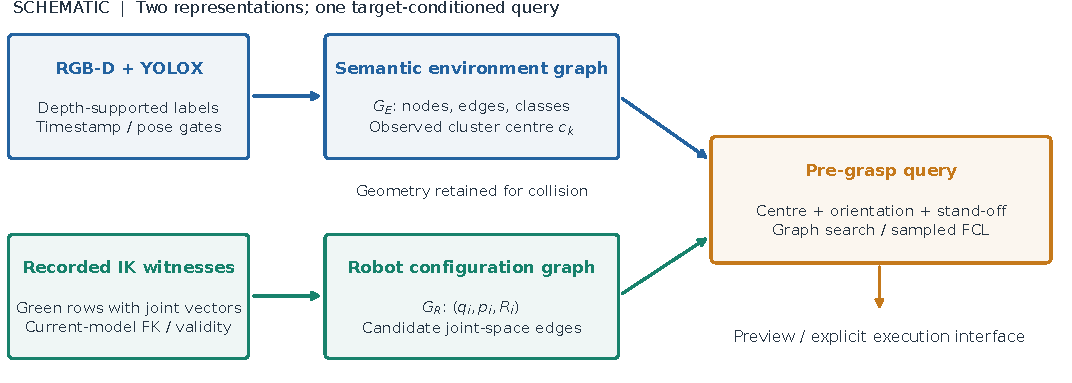
\includegraphics[width=\textwidth]{architecture.pdf}
\caption{Architecture schematic, not an experimental trajectory. The environment graph supplies semantic components and observed collision geometry. The robot graph supplies full pose and joint witnesses. Target-conditioned queries connect them through geometric eligibility and motion validation.}
\label{fig:architecture}
\end{figure*}

\subsection{Local Alignment Versus Side Approach}
Equation~\eqref{eq:alignment} asks whether the configured tool axis faces the object. It allows a pose above the object with a downward-facing tool. A side approach needs a separate world-frame directional requirement. For example, given desired horizontal direction $h_k$ and world vertical $e_z$, a possible additional contract is
\begin{equation}
 (R_i a_T)^\top h_k\ge\cos\epsilon_h,\qquad
 |(R_i a_T)^\top e_z|\le\sin\epsilon_z.
 \label{eq:horizontal}
\end{equation}
One can also constrain $(c_k-p_i)/d_{ik}$ to the same horizontal cone. For radial approach, $h_k$ can point from the base toward $c_k$ after projection onto the horizontal plane. Equations~\eqref{eq:horizontal} describe an extension to evaluate; the audited default planner enforces Eq.~\eqref{eq:alignment}, not these horizontal constraints. Figure~\ref{fig:geometry} illustrates why moving the target to the center alone cannot select a side approach.

\section{System and Query Procedure}
\subsection{Semantic Environment Topology}
The perception pipeline uses a wrist-mounted RGB-D sensor, YOLOX, robot kinematics, and a world-frame DD-GNG backend. Native depth geometry is transformed using the camera extrinsics and available robot transforms; a robot-body mask removes modeled self observations. Invalid depth cannot become a metric target simply because the RGB detector recognizes an object. The current empirical vertical offset is a local calibration correction, not evidence of a globally accurate camera-to-robot transform.

The semantic-attention backend assigns directly supported regions a strength $S=1+(S_{\max}-1)\gamma$, with $S_{\max}=3$ and a fused semantic score $\gamma$. Overlap uses maximum strength, not accumulated strength. Up to half the update samples are drawn from attended regions, with the remainder drawn over the accepted cloud. Split priority uses $ES^4$, where $E$ is node error, and utility influences recycling at capacity. These are implementation choices based on DD-GNG~\cite{saputra2023ddgng}; the retained global sample quota does not guarantee sufficient representation of every obstacle.

Detector results carry input-sequence and receipt-time information. The documented default guards withhold association after 1.0~s, 0.02~m of camera translation, or 0.10~rad of camera rotation from the source pose. Attention expires according to source receipt time. These guards bound use of stale detections but do not recover exact exposure timestamps or compensate for independently moving objects.

An unknown node may inherit a class from at least two directly connected, sufficiently confident neighbors within 0.055~m when no competing class supplies support. Updates are simultaneous, avoiding a cascade within the same update. These completed labels affect visualization and planning-component membership, but do not become direct detector evidence for attention. They do not repair conflicting detector assignments or supply ground-truth instance segmentation. The complete observed point-and-edge geometry is retained for collision modeling regardless of target coloring.

\subsection{Importing Configuration Witnesses}
The separate experiment launch selects archived rows with both numerical success flags set and categorical status \texttt{pose\_found}. Near-singular rows also have the numerical full-pose flag set, so flag-only selection would admit a different bank. Every retained row provides six joint values and a requested Cartesian position. The importer recomputes the actual pose with the current URDF, checks finite values, joint limits, and the configured self-collision predicate, and removes duplicate configurations. Nearby Cartesian points with distinct retained joint vectors need not collapse to one vertex.

Candidate edges are proposed using normalized joint distance
\begin{equation}
 d_Q(q_i,q_j)=\sqrt{\sum_{a=1}^{6}
 \left(\frac{q_{i,a}-q_{j,a}}{q_a^{\max}-q_a^{\min}}\right)^2}.
\end{equation}
The experiment reuses the existing local connection limits: ten candidate neighbors, $d_Q\le0.75$, and end-effector displacement at most 0.14~m. The workspace backend's candidate adjacency is not a certificate that every edge is collision-free in the current scene. A measured-start connector is separately checked before query traversal.

\subsection{Collision-Checked Search}
All observed nodes and edges, including the selected object, can enter the complete collision scene as spheres and cylinders. Cached or on-demand body capsules provide preliminary rejection. Detailed robot-mesh checks use MoveIt/FCL at interpolated joint states. In the default experiment profile the exact-transition spacing bounds the largest joint increment by 0.05~rad. Calling this check ``exact'' in the implementation distinguishes the geometry backend from capsule approximation; it does not establish continuous-time safety between the samples.

For a fixed object component, the intended query contract is as follows. The current prototype implements the search and validation stages; the atomic target/preview binding still has the limitations identified in Section~VI.
\begin{enumerate}
\item Freeze the environment observation, target identity, center, robot-model configuration, and measured start used for the query.
\item Select eligible pre-grasp vertices using Eqs.~\eqref{eq:alignment}--\eqref{eq:relation}; remove those rejected by current node checks.
\item Connect the measured start to an admissible roadmap vertex and search the enabled graph for a reachable eligible goal.
\item Check every proposed transition against the current collision scene. Disable a rejected candidate edge and repeat search within the budget.
\item Optionally replace a subsequence with a directly interpolated joint transition only after checking that replacement against the same scene.
\item Publish a pose/joint-path preview, chosen target, and validation diagnostics for review.
\end{enumerate}
The implementation first favors geometric proximity of reachable eligible goals to the target and uses joint-path cost to break ties. It therefore should not be described as optimizing a globally shortest Cartesian approach. Shortcutting may add checked transitions absent from the original edge set, so the resulting trajectory follows an \emph{augmented} graph rather than necessarily every original graph edge.

\subsection{Execution Boundary}
The coordinator associates the target with an object track, freezes a preview, and checks perception freshness, joint-state availability, calibration status, controller availability, and execution settings. Its default experiment task is \texttt{move\_to\_target}; it does not close the gripper. The controller architecture can add a teleoperation offset to the automatic position reference. Such offsets change the actual path and must be accounted for in any execution validation; a nominal preview alone cannot validate arbitrary manual corrections.

These checks constitute an implementation interface, not a formal execution guarantee. The current frozen-plan path must still be audited for equality between the validated and transmitted start/path states. We report no proof of payload-aware motion, dynamic-obstacle avoidance, or safe concurrent teleoperation. A complete pickup sequence also needs a contact-aware final approach and a lift trajectory; simply closing the fingers at a stand-off pose is insufficient.

\begin{figure*}[t]
\centering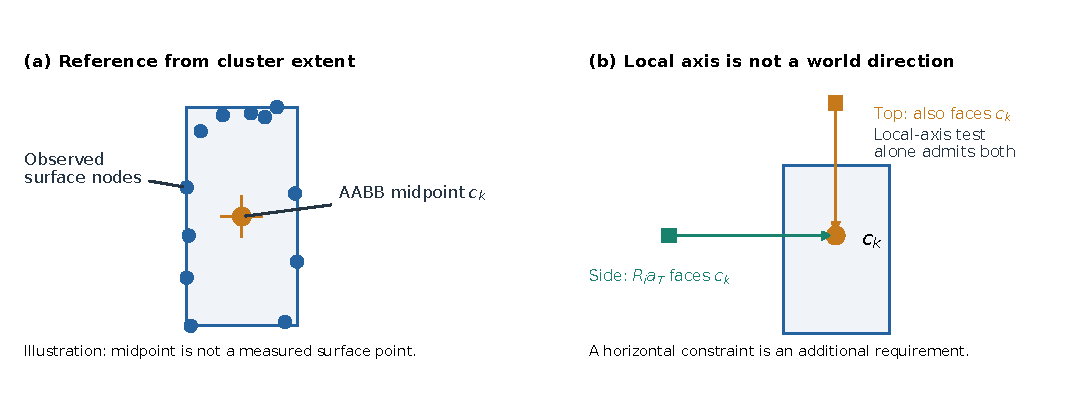
\includegraphics[width=\textwidth]{target_geometry.pdf}
\caption{Target and orientation schematic. (a) The selected point is the midpoint of observed component bounds, independent of which surface node represents its identity. (b) Both a side-facing and a downward-facing axis can satisfy an axis-to-center alignment test. Desired approach direction in the world frame is an additional constraint.}
\label{fig:geometry}
\end{figure*}

\section{Offline Evidence and Frame Audit}
\subsection{Dataset and Scope}
We reanalyze the archived V2 workspace scan on a 25~mm Cartesian grid within a 0.5~m sphere. The scan contains 33,401 requested positions and uses bounded multi-start Levenberg--Marquardt IK, recorded position/orientation tolerances, a conditioning threshold, and an endpoint capsule collision model. The scan is a numerical model experiment. Its rows are neither independent physical trials nor complete statements about the robot's reachable workspace: a failed bounded search does not prove unreachability, and a successful endpoint does not prove a feasible motion from an arbitrary start.

The analysis script reads the original CSV without editing it, verifies mutually exclusive status counts, reports selection fractions, and records the file hash and scanner provenance. Historical synthetic-planning benchmarks from another roadmap construction and earlier perception code are excluded. Instrumentation-only recordings are not counted as successful object-manipulation trials.

\begin{table}[t]
\centering\caption{Archived offline workspace outcomes. Counts describe the scanner's bounded search, not physical execution success.}
\label{tab:workspace}
\small\begin{tabular}{@{}lr@{}}\toprule
Recorded category & Grid queries \\\midrule
Nonsingular full pose (green) & 3,198 \\
Near-singular full pose (blue) & 334 \\
Position found, orientation unresolved & 11,643 \\
Position unresolved & 17,868 \\
Collision candidates only & 358 \\\midrule
Total & 33,401 \\\bottomrule
\end{tabular}
\end{table}

\subsection{Position Support Is Not Pose Support}
Table~\ref{tab:workspace} gives the exact category counts. A position witness was recorded for 15,175 queries. The selected green subset contains 3,198 rows, representing 9.57\% of all grid queries and 21.07\% of position-witness queries. There are 3,532 numerical full-pose successes if near-singular rows are included. The green selection intentionally excludes 334 of them.

Among the selected rows, the largest recorded position residual is 0.9997~mm and the largest orientation residual is approximately $0.43961^\circ$. These are residuals against the scanner's target pose and URDF, not camera calibration error or physical TCP accuracy. Figure~\ref{fig:workspace} visualizes the selected positional support. Its appearance cannot reveal the missing orientation dimension. The selected-row count also differs conceptually from the number of vertices accepted after current-model import and deduplication.

\begin{figure}[t]
\centering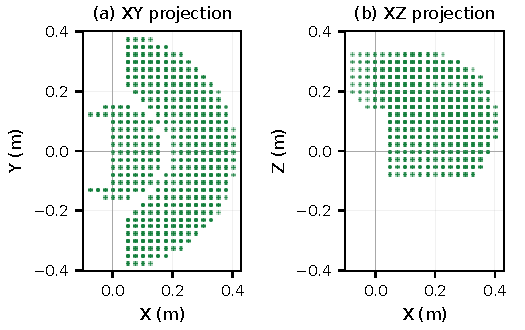
\includegraphics[width=\columnwidth]{workspace_audit.pdf}
\caption{Positions of archived green witnesses, projected into workspace planes. Generated from the recorded CSV, not a live robot run. Multiple projected points can overlap; the plot does not imply arbitrary orientation availability or collision-free connectivity.}
\label{fig:workspace}
\end{figure}

\subsection{The Scan's Frame Conversion}
Let $G$ denote the gripper orientation convention used by the scan, and $T$ the end-effector frame used by forward kinematics. The scanner contains the fixed matrix
\begin{equation}
 A={}^TR_G=\begin{bmatrix}0&0&-1\\0&1&0\\1&0&0\end{bmatrix},
 \qquad {}^WR_T={}^WR_G A^\top.
 \label{eq:conversion}
\end{equation}
For the archived radial policy, gripper roll and pitch are zero and yaw is $\psi=\operatorname{atan2}(y,x)$, so ${}^WR_G=R_z(\psi)$. Multiplying the basis vectors gives
\begin{align}
 {}^WR_T e_x&=-e_z, \label{eq:down}\\
 {}^WR_T e_z&=(\cos\psi,\sin\psi,0)^\top.\label{eq:front}
\end{align}
Thus horizontal gripper-frame $+X$ corresponds to end-effector-frame $+Z$ under this conversion, while end-effector-frame $+X$ points downward. We independently reconstructed the frozen URDF chain using an XML parser and NumPy rigid transforms, and evaluated every selected six-joint witness. All 3,198 configurations reproduced the recorded pose residuals within numerical precision. Their actual local-$+X$ axes deviated from world-down by at most $0.439607^\circ$ (Table~\ref{tab:frames}). This verifies the numerical witnesses under the archived model, not the physical gripper calibration or the active live planner state.

This provides a mechanism consistent with an apparently misleading visualization: a rich bank of green Cartesian points can keep yielding downward local-$+X$ arrows. The arrow can correctly depict the selected pose while the configured approach axis is wrong for the intended physical frame. A change of marker color or target-node identity cannot resolve the mismatch. Mechanical verification of the frame definition is needed before choosing the corrected local axis or regenerating orientation-diverse samples. Runtime imports recompute FK from the current model, so a claim about a particular live trajectory additionally requires its model and selected joint path.

\begin{table}[t]
\centering\caption{Independent FK of all 3,198 selected witnesses using the archived URDF. Rounded maxima; no physical measurements.}
\label{tab:frames}
\small\begin{tabular}{@{}lr@{}}\toprule
Quantity & Maximum \\\midrule
Local $+X$ angle from world-down & $0.439608^\circ$ \\
Local $+Z$ angle from horizontal & $0.439608^\circ$ \\
$|(R_i e_z)^\top e_z|$ & 0.007673 \\
Position-residual discrepancy & $1.22\!\times\!10^{-13}$ mm \\
Rotation-residual discrepancy & $2.36\!\times\!10^{-14}$ deg \\\bottomrule
\end{tabular}
\end{table}

\subsection{A Bound on Horizontal Local-$+X$ Alignment}
Let $h$ be any horizontal unit direction. If an actual witness differs from the target orientation by at most $\epsilon$, Eq.~\eqref{eq:down} implies
\begin{equation}
 |(R_i e_x)^\top h|\le\sin\epsilon.
 \label{eq:bound}
\end{equation}
Using the largest selected-row residual, $\epsilon<0.44^\circ$, yields an upper bound below 0.0077, far below the configured alignment threshold 0.70. Therefore this witness bank cannot support a truly horizontal target direction under a local-$+X$ goal predicate, within the recorded model residuals. It can still supply aligned goals \emph{above} a target. This is a frame-and-orientation limitation, not evidence that the target position lies outside the arm's workspace.

The radial direction in Eq.~\eqref{eq:front} is also a restricted orientation policy. Correcting a frame-axis mismatch would not establish arbitrary yaw, roll, or obstacle-dependent approach coverage. A task-conditioned witness bank must retain multiple validated orientations when the manipulation task requires them.

\section{Limitations and Required Evaluation}
\subsection{Implementation Gaps}
The current planner combines pre-grasp eligibility into a union of robot-node flags across target components. A node eligible for one component can subsequently be associated with another unless the pairwise predicate is checked again. Equation~\eqref{eq:relation} makes the required relation explicit. Until that behavior is corrected and tested, conclusions about object-conditioned planning must be restricted to a single selected component; a multi-object correctness claim would be premature.

The coordinator recomputes the cluster center from an associated environment snapshot rather than consuming an authoritative frozen center carried in the plan. Snapshot association therefore does not alone establish equality of the planned and displayed target. An improved message contract should bind component membership, center, scene revision, approach-frame convention, and joint trajectory to the same query. This is a required integration refinement, not a measured result.

The collision model is also incomplete. It approximates observed geometry with primitives, cannot cover unobserved surfaces, and uses sampled joint transitions. The experiment has an explicit self-contact exemption for one link pair and omits part of the fixed-base environment interaction. Gripper state and carried objects require consistent modeling. These limitations preclude interpreting graph connectivity or successful preview as a blanket collision-safety guarantee.

\subsection{Proposed Controlled Study}
The next evaluation should freeze camera extrinsics, frame conventions, model version, witness-bank hash, object layout, and source revision before collecting comparative results. We propose four matched policies: individual labeled-node targets with position-only eligibility; observed-cluster-center targets with position-only eligibility; centers with correctly expressed tool-axis eligibility; and centers with both tool-axis and horizontal-cone constraints. All policies must use identical observations, candidate configurations, connection budgets, and collision predicates. A second factor compares the existing orientation-specific bank with a new bank containing multiple orientations per position.

Scene resets should include one and two instances, bottle--keyboard image-box overlap, partial occlusion, and varied start configurations. To avoid confounding adaptive graph memory with the policy, each comparison should replay a frozen observation or reset the learner identically. Ground-truth cluster membership and reference targets must be independently annotated or measured. A center defined only from the same predicted labels cannot be its own segmentation ground truth.

Report correct-component selection, target displacement, eligible-pair count, start-connected goal rate, sampled-collision-valid plan rate, target-direction error, latency, and diagnostic failures. Failed detection or target selection must remain in end-to-end denominators. For repeated layouts, uncertainty should resample complete scene resets, preserving within-scene dependencies. Compare against a conventional planning baseline under the same terminal constraints and collision scene; differences in collision models or goal tolerances must not masquerade as planning improvements.

Only after pose and execution consistency are checked should physical outcomes be measured separately: approach reached, contact-aware insertion completed, fingers closed, object lifted, and object placed. Manual offsets should be logged as interventions and analyzed independently from nominal autonomous executions. None of these outcomes has been established by the offline scan or the screenshots motivating this manuscript.

\section{Conclusion}
Cluster-centered dual-graph planning separates what the object is, where its observed geometric reference lies, and which robot configuration can approach it. The archived scan supplies 3,198 conditioning-qualified full-pose witnesses; independent FK confirms their local-$+X$ axes are approximately vertical under that model. This finding demonstrates a mechanism by which positional reachability and a center target can coexist with an undesired overhead approach. The next step is to verify the physical frame convention, preserve target-conditioned eligibility through the full query, and evaluate pose coverage and task execution under controlled scenes. No conclusion about autonomous grasp success follows from the current evidence.

\section*{Acknowledgments and AI Disclosure}
OpenAI Codex (GPT-6) assisted with drafting all manuscript sections, source-code and data inspection, and the analysis and figure scripts. Numerical results derive from archived data; the architecture and target-geometry drawings are labeled schematics. This draft requires human author review of all claims and citations before submission.

\bibliographystyle{IEEEtran}
\bibliography{references}
\end{document}
